\documentclass[11pt]{article}
\usepackage[margin=18mm]{geometry}
\usepackage{booktabs,graphicx,hyperref}
\begin{document}
\title{Event analysis: paired scans and ensemble means}
\author{NAUSICAA}\date{}\maketitle
This checkpoint retains the approved baseline and evaluates numerical/selection
changes on the same events. Julia computes all counts, decisions, paired metrics
and ensemble reductions. The cumulative core suite passes 2066 assertions.

\section*{Ensemble convention and denominators}
The pad containing the selected track's energy-weighted x/y reference becomes
the central pad, with centre at (0,0). This relabels existing physical pads and
preserves integer counts. The relative arrival axis starts at each history's
first saved arrival edge. The configured direction is retained. Every accepted
event contributes its full retained diffusion charge; all cells and zero-count
intervals are represented by the saved axes.

The same exact integer numerator is divided by two explicit denominators:
accepted events, and all processed events (with rejected events contributing
zero selected charge). The means use Float32. With no accepted events, the
conditional mean is undefined (NaN) and the processed mean is zero. The HDF5
stores numerator, both denominators, both means, axes and alignment metadata.
\begin{center}\small\begin{tabular}{lrrr}\toprule
Sample & Accepted/processed & Ions/accepted event & Selected ions/processed event \\\midrule
Double beta & 22/50 & 112213.4 & 49373.9 \\
Electron background & 31/50 & 112077.3 & 69487.9 \\
\bottomrule\end{tabular}\end{center}
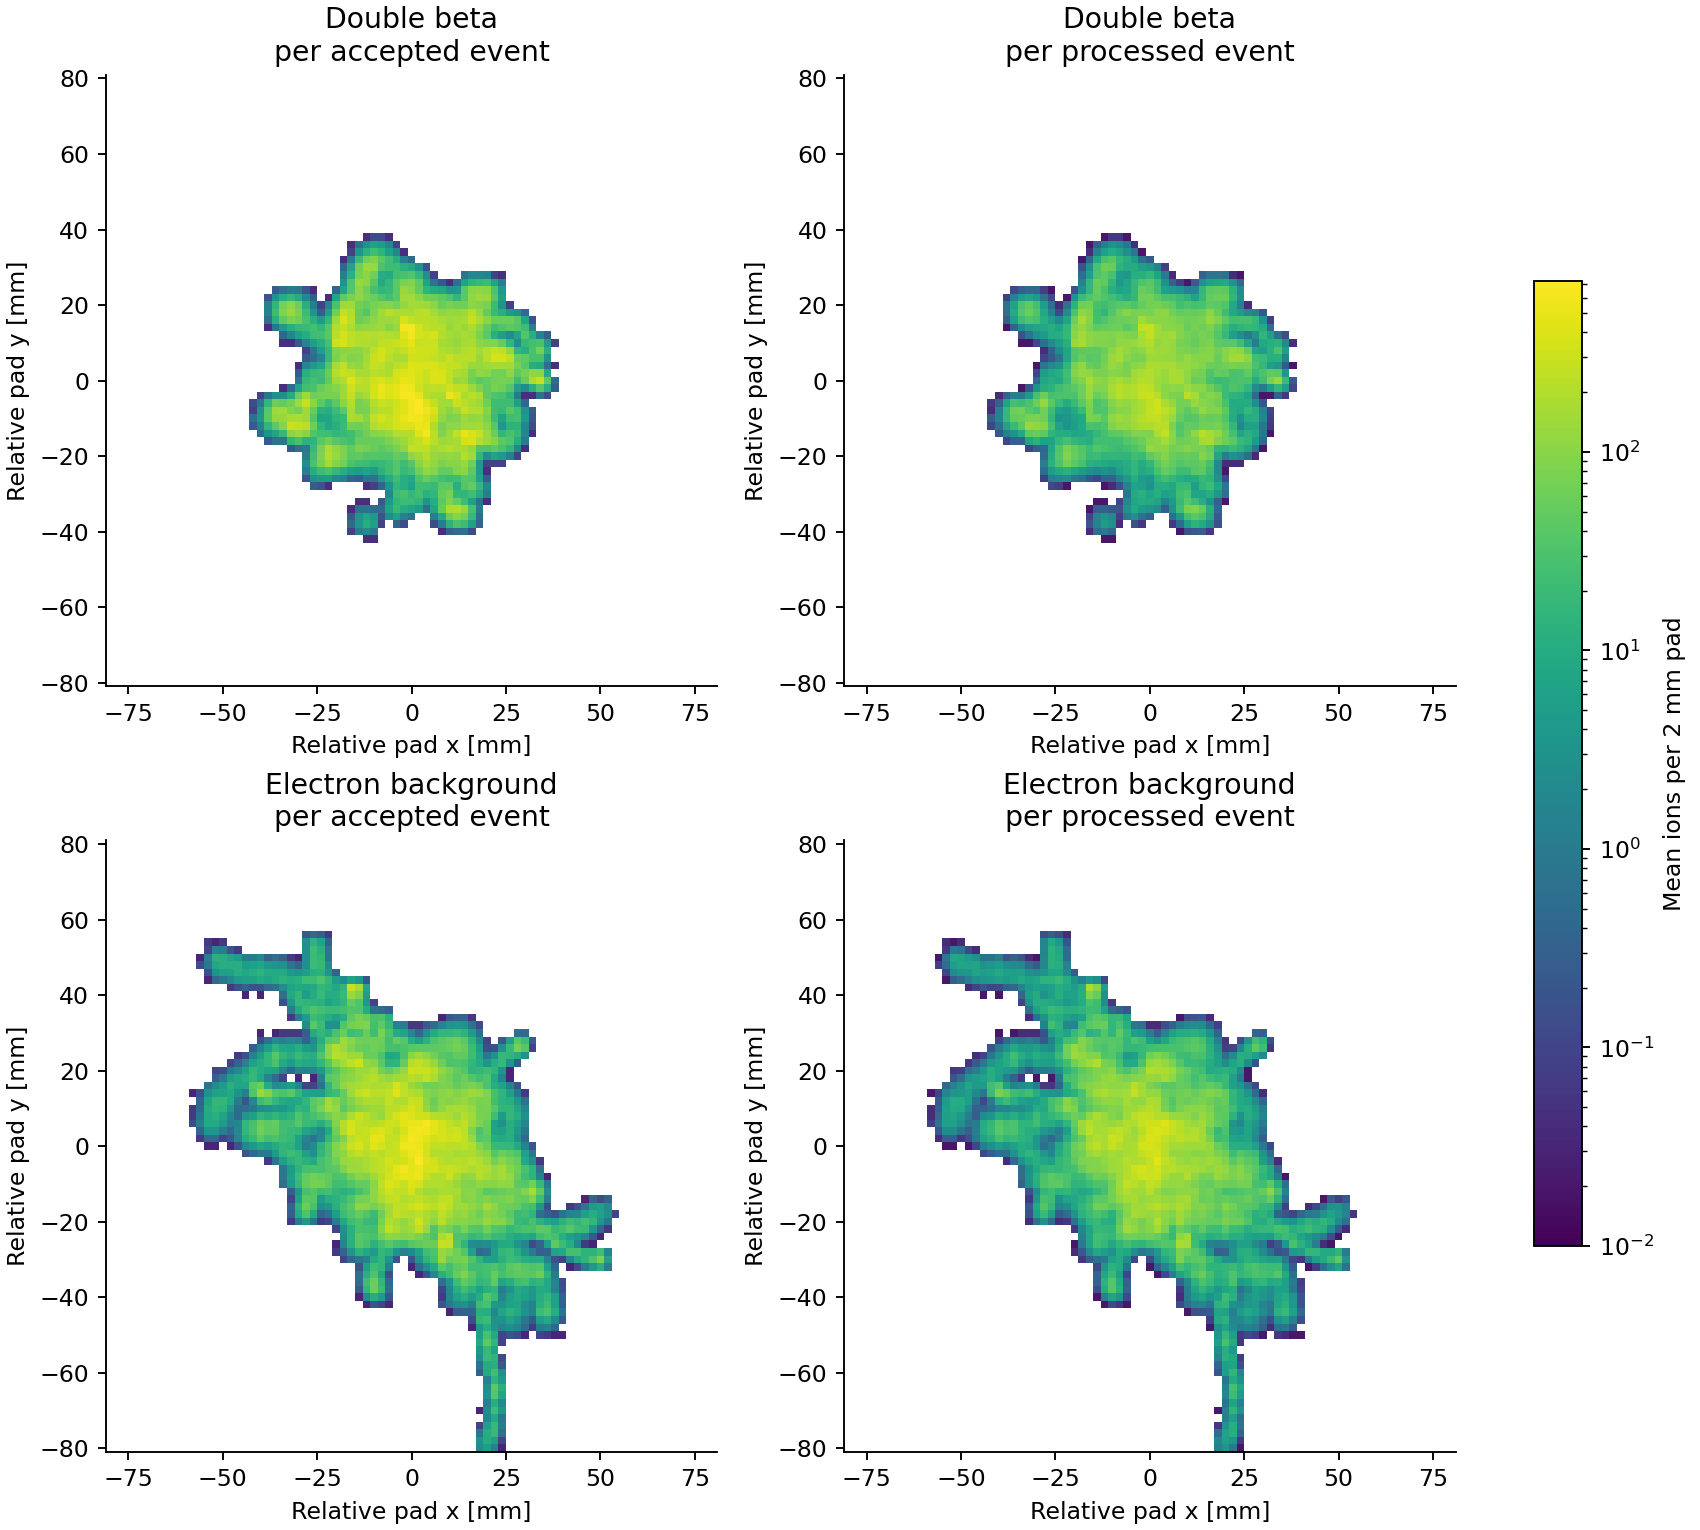
\includegraphics[width=\linewidth]{ensemble_xy.png}
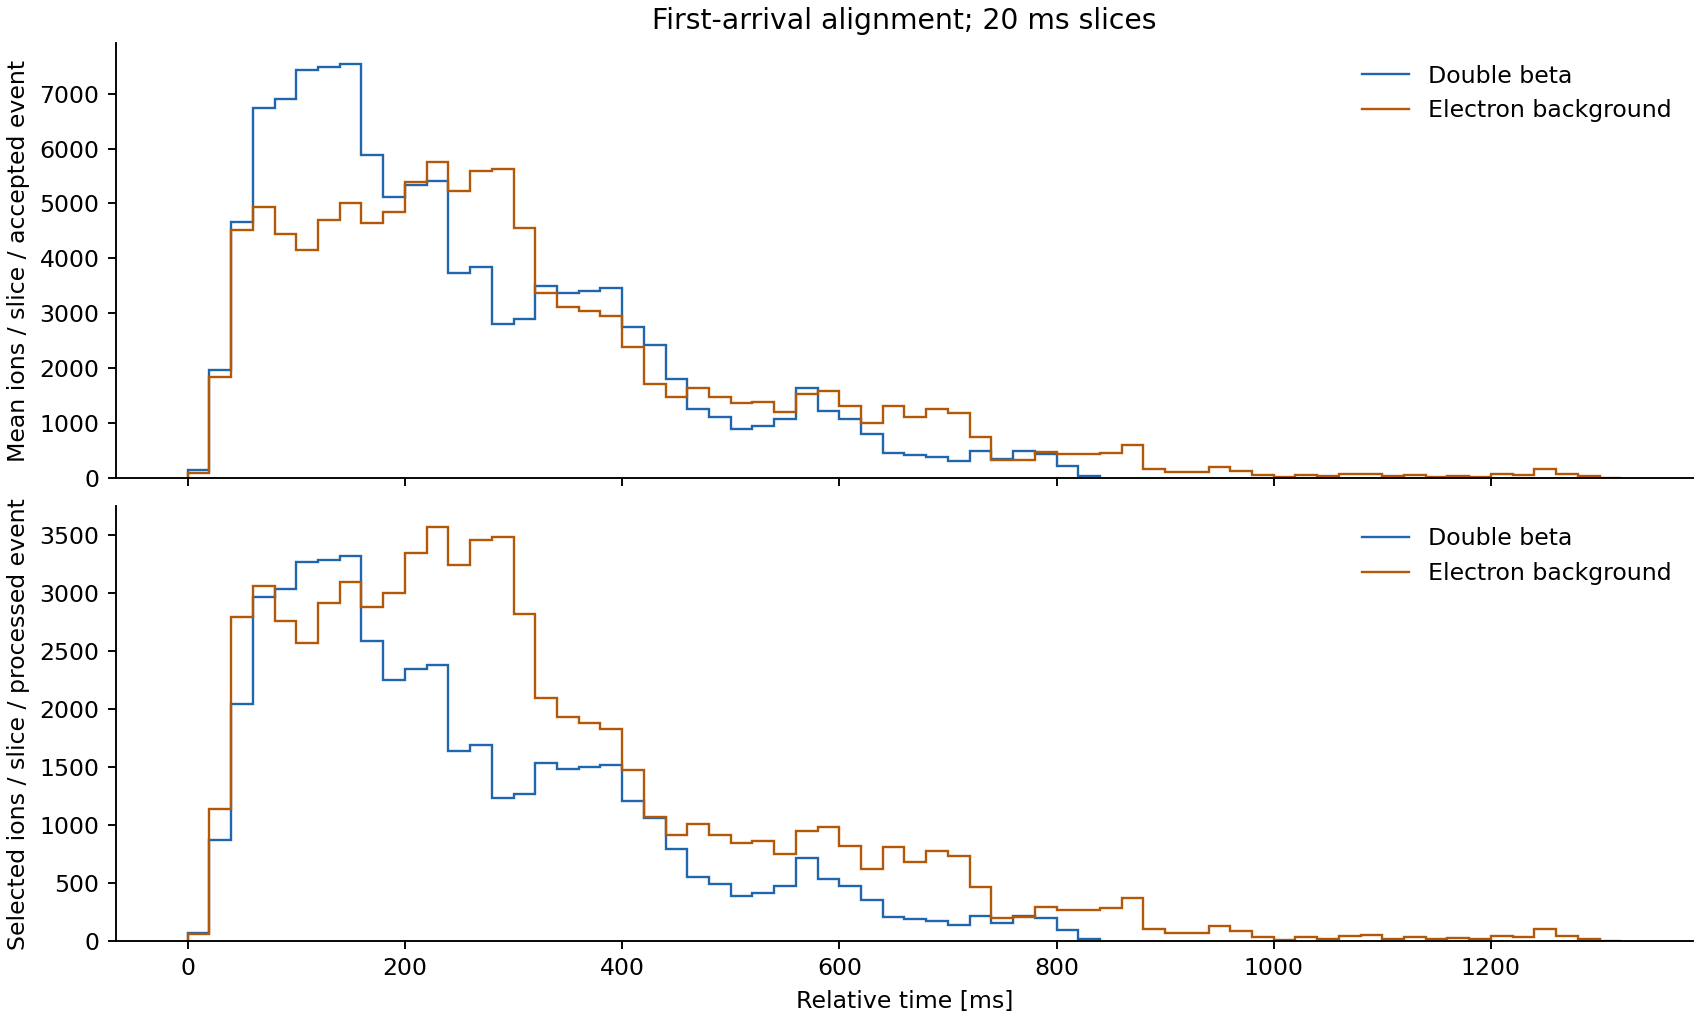
\includegraphics[width=\linewidth]{ensemble_time.png}

\section*{Paired scan design}
Each variation changes one setting family from the baseline: diffusion histogram
bin count, Gaussian padding, kNN neighbour count, ion threshold or a common
multiplier of both the $3\sigma_T$ bin width and $6\sigma_T$ edge cutoff. Drift,
ion draws and grid offsets are paired by saved stage seeds. Graph-only variants
reuse the same diffusion table. Changing histogram bin count at fixed bounds
preserves every retained ion; this is checked for each event.

Lost and gained refer to the same baseline event decisions, so equal acceptance
counts cannot conceal exchanged events. Shared counts give the denominator for
the paired pad metric. This subset is a validation sample, not a full-sample
efficiency determination. Baseline cuts remain unchanged.

\section*{Pad-response comparison}
For paired count tables A and B, use $D=\sum|A-B|/(\sum A+\sum B)$: zero means
identical charge allocation; one means disjoint allocation. The Full comparison
uses each variant's reconstructed grid reference and first-arrival alignment.
The Fixed comparison collects both diffusion tables on the baseline accepted
track's physical lattice, using signed cell indices to eliminate coverage and
time-origin relabelling. Graph-only changes therefore have zero Fixed distance.
These distances measure redistribution, not lost total charge.
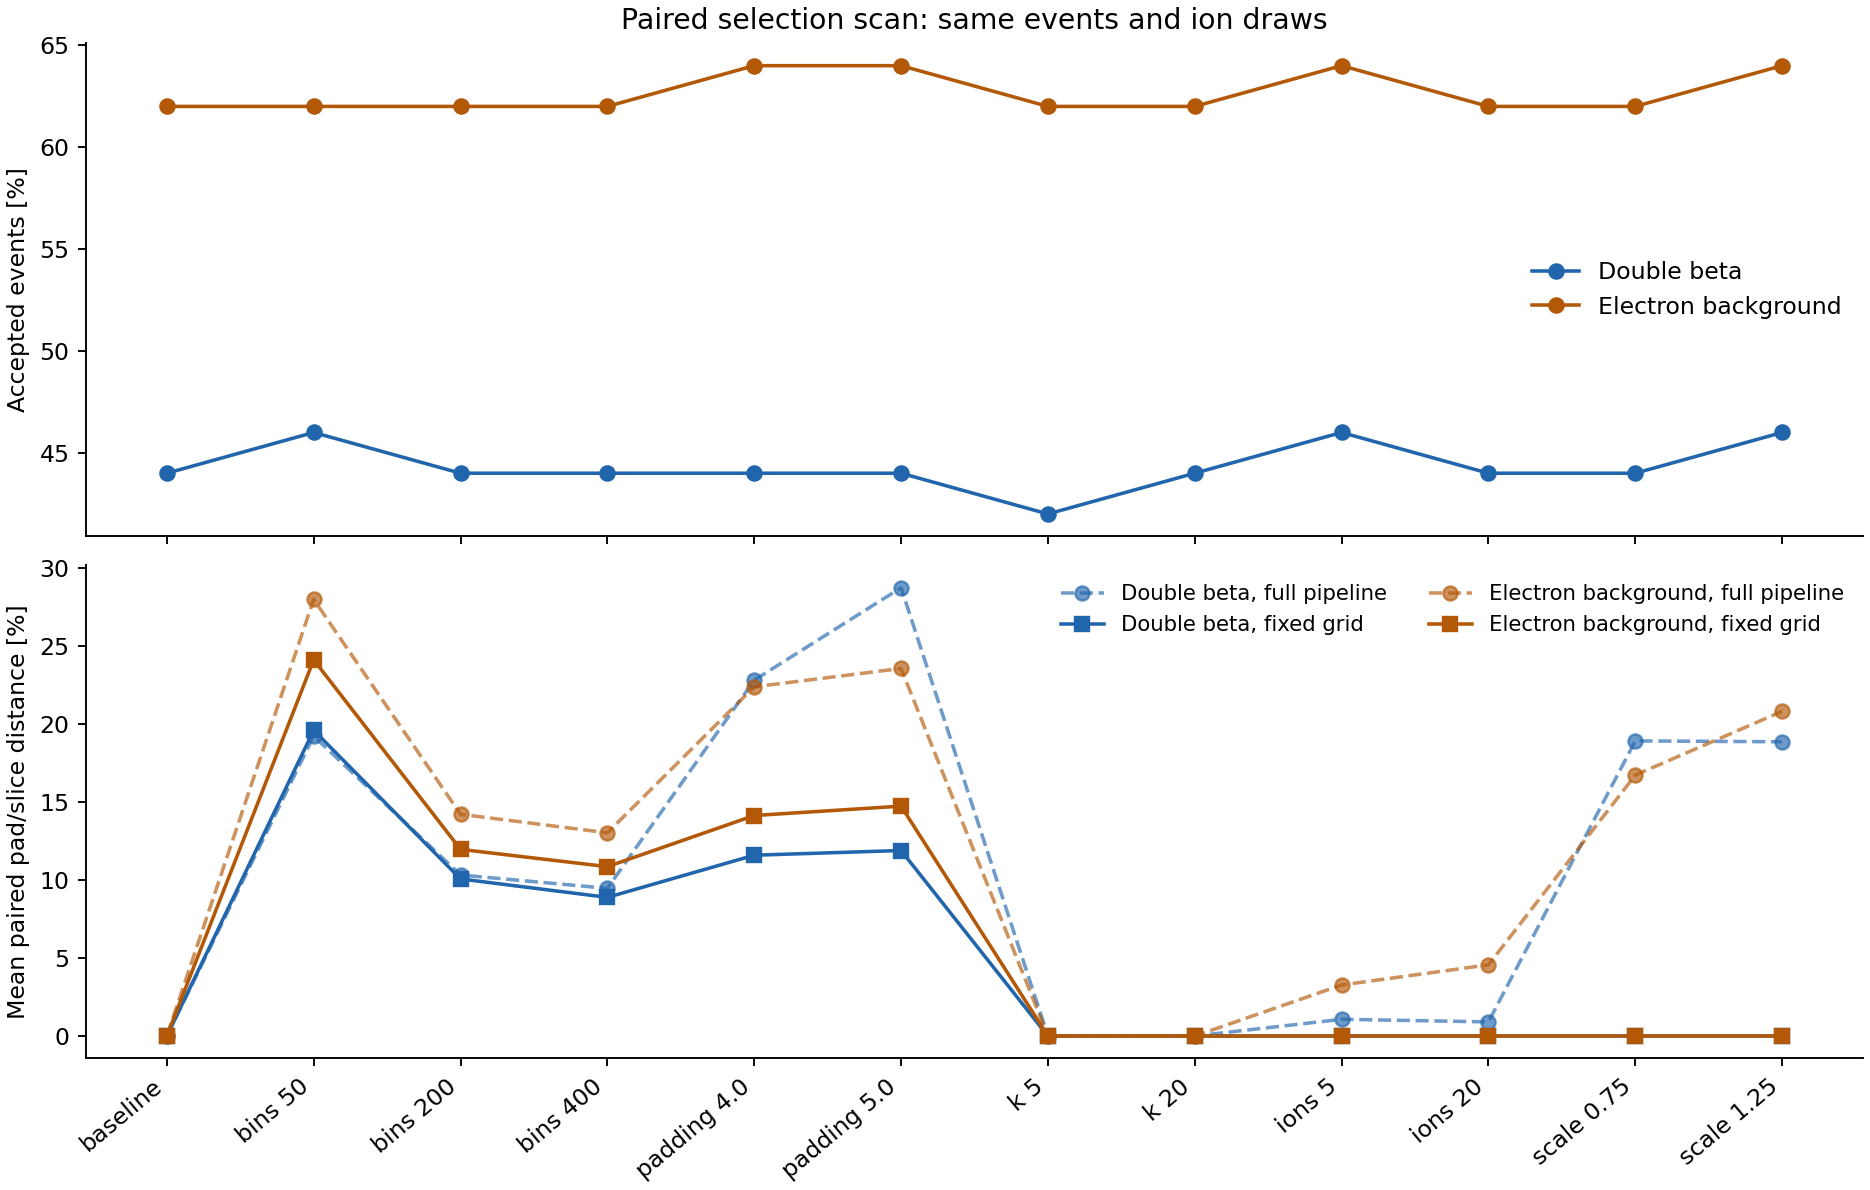
\includegraphics[width=\linewidth]{paired_scans.png}
\subsection*{Double beta}
\begin{center}\small\begin{tabular}{lrrrrrr}\toprule
Variant & Pass & Lost & Gained & Shared & Full [\%] & Fixed [\%] \\\midrule
baseline & 22 & 0 & 0 & 22 & 0.00 & 0.00 \\
bins\_50 & 23 & 0 & 1 & 22 & 19.22 & 19.59 \\
bins\_200 & 22 & 0 & 0 & 22 & 10.32 & 10.07 \\
bins\_400 & 22 & 0 & 0 & 22 & 9.47 & 8.89 \\
padding\_4.0 & 22 & 0 & 0 & 22 & 22.80 & 11.59 \\
padding\_5.0 & 22 & 0 & 0 & 22 & 28.73 & 11.89 \\
k\_5 & 21 & 1 & 0 & 21 & 0.00 & 0.00 \\
k\_20 & 22 & 0 & 0 & 22 & 0.00 & 0.00 \\
ions\_5 & 23 & 0 & 1 & 22 & 1.07 & 0.00 \\
ions\_20 & 22 & 0 & 0 & 22 & 0.91 & 0.00 \\
scale\_0.75 & 22 & 0 & 0 & 22 & 18.91 & 0.00 \\
scale\_1.25 & 23 & 0 & 1 & 22 & 18.86 & 0.00 \\
\bottomrule\end{tabular}\end{center}
\subsection*{Electron background}
\begin{center}\small\begin{tabular}{lrrrrrr}\toprule
Variant & Pass & Lost & Gained & Shared & Full [\%] & Fixed [\%] \\\midrule
baseline & 31 & 0 & 0 & 31 & 0.00 & 0.00 \\
bins\_50 & 31 & 0 & 0 & 31 & 27.98 & 24.10 \\
bins\_200 & 31 & 0 & 0 & 31 & 14.21 & 11.96 \\
bins\_400 & 31 & 0 & 0 & 31 & 13.02 & 10.85 \\
padding\_4.0 & 32 & 0 & 1 & 31 & 22.38 & 14.13 \\
padding\_5.0 & 32 & 0 & 1 & 31 & 23.55 & 14.73 \\
k\_5 & 31 & 0 & 0 & 31 & 0.00 & 0.00 \\
k\_20 & 31 & 0 & 0 & 31 & 0.00 & 0.00 \\
ions\_5 & 32 & 0 & 1 & 31 & 3.27 & 0.00 \\
ions\_20 & 31 & 0 & 0 & 31 & 4.56 & 0.00 \\
scale\_0.75 & 31 & 0 & 0 & 31 & 16.72 & 0.00 \\
scale\_1.25 & 32 & 0 & 1 & 31 & 20.81 & 0.00 \\
\bottomrule\end{tabular}\end{center}

\section*{Successive histogram resolution checks}
The following comparisons use the same baseline physical lattice and events
accepted in the baseline and both compared settings. The 200-to-400 check was
added after the first scan showed a measurable pad response to resolution.
\begin{center}\small\begin{tabular}{lllrr}\toprule
Sample & Reference & Variant & Shared & Fixed distance [\%] \\\midrule
Double beta & baseline & bins\_200 & 22 & 10.07 \\
Double beta & bins\_200 & bins\_400 & 22 & 5.08 \\
Electron background & baseline & bins\_200 & 31 & 11.96 \\
Electron background & bins\_200 & bins\_400 & 31 & 6.06 \\
\bottomrule\end{tabular}\end{center}
Selection stability and pad-response convergence are evaluated separately.
The results and the required accuracy for pad histories should be reviewed
before selecting production settings and running the complete samples.

\section*{Validation and reproduction}
Tests cover translation-invariant central-pad alignment, both denominators,
missing-event cells as zero, complete axis coverage, integer conservation,
undefined conditional means for zero acceptance, Float32 reduction precision,
HDF5 round trips and corruption detection. Every written ensemble is read back;
its exact numerator matches the persisted aligned histories.
\begin{verbatim}
make validate-event-step4 PYTHON=/path/to/python3.11-or-newer
# Presentation from the saved numerical output:
make report-event-step4 PYTHON=/path/to/python3.11-or-newer
\end{verbatim}
Numerical data, event decisions, aligned histories, paired metrics and provenance:
\par\noindent\path{results/event_analysis/step4_scans.h5}.
\par The ensemble subgroups use schema \texttt{nausicaa.event.ensemble.v1}.
\section*{Configuration used}
\footnotesize\begin{verbatim}
# Event-analysis checkpoints. Detector constants come from the SI card.
[inputs]
detector_card = "config/detector.toml"
samples = ["events/0nubb_hitdf.h5", "events/electron_0nubb_energy_hitdf.h5"]

[ionization]
ionisation_energy_eV = 21.9
# Same adopted nominal W as the initial ion_tracks analysis.

[drift]
min_cm = 10.0
max_cm = 150.0

[diffusion]
longitudinal = "thermal" # "zero" is the longitudinal comparison
nbins = 100
nsigma = 3.0

[graph]
method = "kNN"
k = 10
min_ions_per_bin = 10
bin_sigma_scale = 3.0
edge_sigma_scale = 6.0

[pads]
z_bin_width_mm = 2.0
minimum_xy_span_mm = 160.0
random_grid_offset = true
# Relative-time convention for this checkpoint: increasing z is later.
# Change to -1 for decreasing-z arrival order. t=0 is the first arrival edge.
drift_direction = 1
# Transverse pitch and ion speed are read from the detector card.

[random]
seed = 2026
# Validation uses explicit per-case seeds, stored in its HDF5.

[validation]
events_per_sample = 5
selection_events_per_sample = 50
synthetic_ions = 200000
drift_cm = [10.0, 80.0, 150.0]
bin_counts = [50, 100, 200]
padding_sigma = [2.0, 3.0, 4.0, 5.0]

[ensemble]
alignment = "central_pad"
minimum_half_cells = 40
# Save both accepted-event means and selected charge per processed event.

[scans]
events_per_sample = 50
histogram_bins = [50, 100, 200, 400]
histogram_padding_sigma = [3.0, 4.0, 5.0]
knn_k = [5, 10, 20]
min_ions_per_bin = [5, 10, 20]
# Multiply both 3sigma bin width and 6sigma edge cutoff by this factor.
graph_scale = [0.75, 1.0, 1.25]

\end{verbatim}
\end{document}
